\chapter{Crystallisation}

In this chapter we apply the concepts of both dynamics and structure to investigate the dynamics of ordering. The vibrations of the molecules make the analysis of dynamical structure more difficult with far more noise as a result of the vibrations.

\section{Melting Points}


\begin{table}
    \centering
    \begin{tabular}{ | c  l | S S S S S |}
        \hline
        Molecule & Crystal & {Melting Point} & {$H_\text{amorphous}$} & {$H_\text{crys}$} & {$\Delta H$} & {$\Delta S$} \\ \hline
        \done & p2mg & 0.80 & & & & \\
        \dcon & p2   & 1.90 & & & & \\
        \tri  & p2   & 1.40 & & & & \\
        \hline
    \end{tabular}
\end{table}


\section{Crystallisation Dynamics}


\subsection{Two Phase Systems}

To get around the issues of waiting for a nucleation event to occur to see the growth of a crystal, we can create a two phase system in which the liquid-crystal boundary is already present. This can then be used to observe the growth of the crystal phase on this surface. Using these two phase configurations as the starting point we see crystallisation of the \done molecule~\figref{done crys}. It is interesting to note that the preferred crystal growth direction is at a \SI{45}{\degree} angle to the crystal boundary. Along with the crystal growth at the existing crystal interface there is also the nucleation of large crystals from the liquid, nucleation may be a fairly common event for the \done molecule.

\begin{figure}
    \begin{subfigure}{\textwidth}
        \includegraphics[width=\textwidth]{{{Snowman-0.75-0.637556-1.0-p2mg-1-frame-0000000000}}}
        \caption{Initial configuration of the two phase system for the \done crystal.}
    \end{subfigure}
    \begin{subfigure}{\textwidth}
        \includegraphics[width=\textwidth]{{{Snowman-0.75-0.637556-1.0-p2mg-1-frame-0320000000}}}
        \caption{Final configuration of the two phase system of the \done crystal.}
    \end{subfigure}
    \caption{A two phase system of the \done molecule with the favoured p2mg crystal in the center. The temperature is held at 0.75. Molecules considered as crystalline are coloured according to their orientation such that molecules that are antiparallel will have the same colour, non-crystalline molecules are grey. This system promotes growth at the boundary of the crystal as seen by the expanding region of teal colour.}
    \label{fig:done crys}
\end{figure}

The two phase analysis can also be performed on the \dcon system~\figref{dcon crys}. The order parameter we are using for the \dcon system appears to be less robust than for the \dcon system, \textfigref{dcon crys} shows many false negatives within the crystal system, while there are also more false positives, individual particles deemed as crystalline. However despite the issues with the order parameter we are able to see a growth in crystallisation~\figref{dcon crys fine}, the regions where the ordered phase is lacking orientational order are regions of growth of the crystal. These orientationally disordered regions have to have come from the liquid phase as the crystal phase has all molecules in an antiparallel orientational order. Also like the \sone molecule we observe the spontaneous nucleation of ordered regions.

\begin{figure}
    \begin{subfigure}{\textwidth}
        \includegraphics[width=\textwidth]{{{Snowman-1.60-0.637556-1.637556-p2-1-frame-0000000000}}}
        \caption{Initial configuration of the two phase system of the \dcon molecule.}
        \label{fig:dcon crys init}
    \end{subfigure}
    \begin{subfigure}{\textwidth}
        \includegraphics[width=\textwidth]{{{Snowman-1.60-0.637556-1.637556-p2-1-frame-0320000000}}}
        \caption{Final configuration of the two phase system of the \dcon molecule.}
        \label{fig:dcon crys fine}
    \end{subfigure}
    \caption{Two phase system of the \dcon molecule with the favoured p2 crystal in the center. The temperature of this system is held at 1.60. Molecules considered ordered are coloured according to their orientation while molecule slacking order are grey. Growth of the crystal can be seen as coloured regions lacking the orientational order of the central crystalline region.}
    \label{fig:dcon crys}
\end{figure}

Unlike the \done and \dcon molecules the \tri molecules does not show crystallisation in the two phase system~\figref{tri crys}. The trimer shows small changes on the surface of the crystal between the initial~\figref{tri crys init} and the final~\figref{tri crys fine} configurations however these are more like what would occur at equilibrium, a rearrangement of the surface rather than growth, despite being below the melting point of the crystal phase. One explanation for this behaviour is the timescale that we are looking at is short compared to the rate of crystal growth.

\begin{figure}
    \begin{subfigure}{\textwidth}
        \includegraphics[width=\textwidth]{{{Trimer-1.30-0.637556-1.00-120-p2-1-frame-0000000000}}}
        \caption{Initial configuration of the two phase system of the \tri molecule.}
        \label{fig:tri crys init}
    \end{subfigure}
    \begin{subfigure}{\textwidth}
        \includegraphics[width=\textwidth]{{{Trimer-1.30-0.637556-1.00-120-p2-1-frame-0320000000}}}
        \caption{Final configuration of the two phase system of the \tri molecule.}
        \label{fig:tri crys fine}
    \end{subfigure}
    \caption{Two phase system of the \tri molecule with the favoured p2 crystal in the central region. The temperature of this system is held at 1.30. Molecules considered ordered are coloured according to their orientation such that molecules that are antiparallel are coloured the same while non-crystalline regions are grey. Despite being below the melting point of the crystal there is no significant net growth of the crystal phase.}
    \label{fig:tri crys}
\end{figure}

\subsection{Spontaneous Nucleation}

We have seen spontaneous nucleation from both the \done and \dcon molecules in the two phase system. We want to be able to see this nucleation from a random starting phase, to show that this is not just a remnant of order from the crystal the liquid phase was melted from. To see this nucleation we had to run simulations far longer than the simulations for dynamics.

The \done molecule shows significant regions of crystallinity~\figref{done nuc}. The configuration is dominated by a number of peach coloured crystals, the dominance of this orientation can be explained by examining the bottom right corner, between above the crystal there are layers of molecules with a more complex ordered structure, this structure forms most of the links between the peach crystal regions keeping them aligned. The other interesting feature of the crystal structure is the boundary between the lavender and peach~\cite{munroe:10} regions where the molecules alternate the crystal structure they are a part of, like a zipper connecting these two crystal regions.

\begin{figure}
    \includegraphics[width=\textwidth]{{{Snowman-0.75-0.637556-1.0-frame-2147000000}}}
    \caption{}
    \label{fig:done nuc}
\end{figure}

\begin{figure}
    \centering
    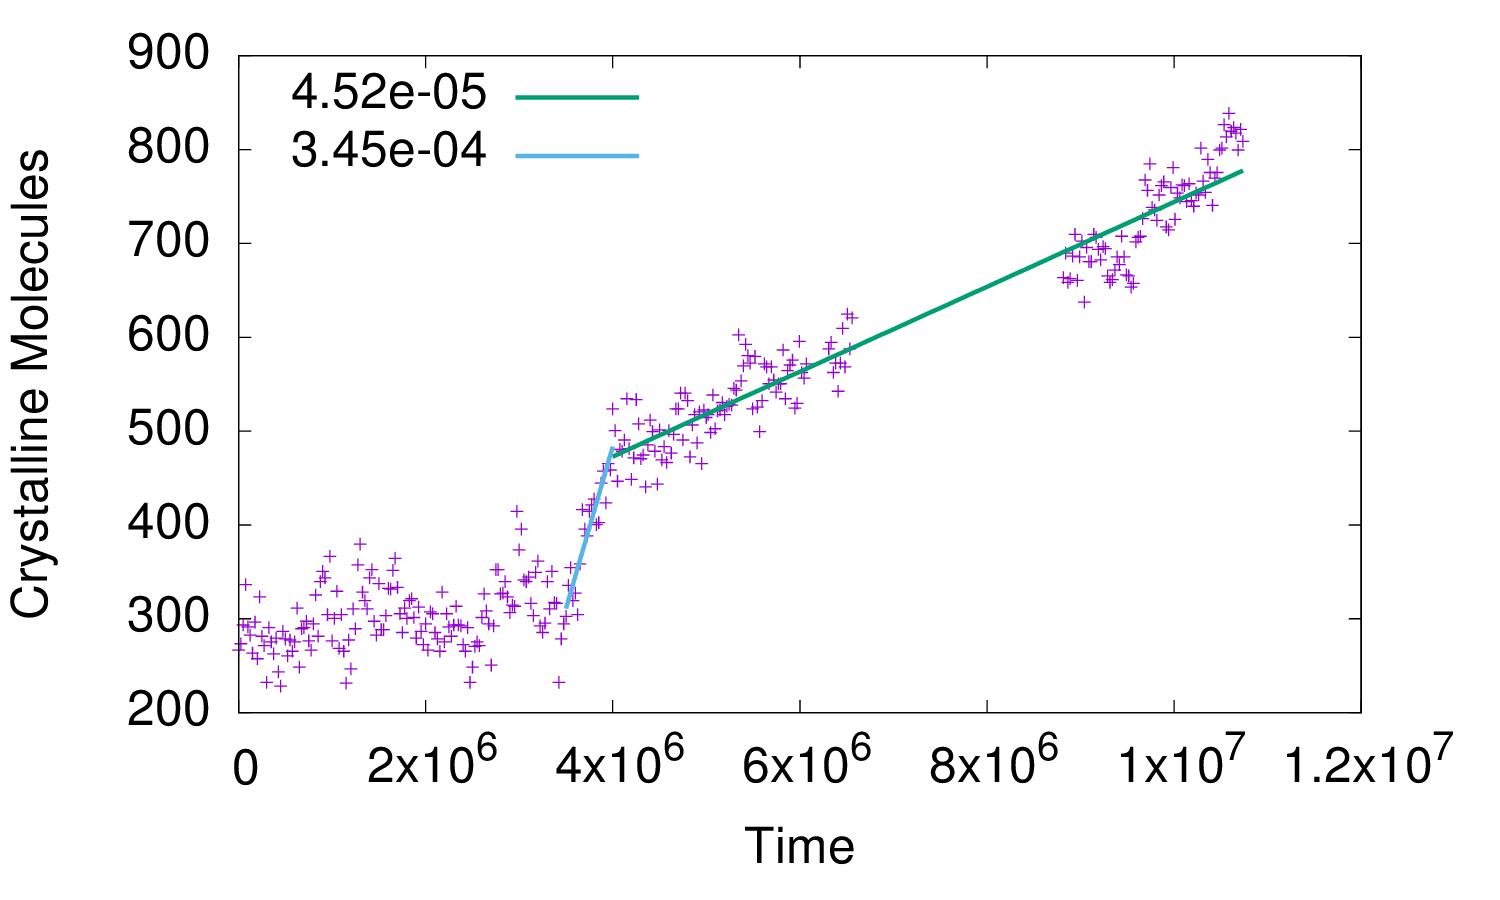
\includegraphics[width=0.5\textwidth]{done_crys_growth}
    \caption{Crystal growth of the \sone molecule. The region of growth can be fitted with a line of gradient \num{1.434e-8}.}
\end{figure}

